\documentclass{article}

\usepackage{graphicx}
\usepackage{multirow}
\usepackage{color}
\usepackage[citecolor=black,linkcolor=black,urlcolor=blue,colorlinks=true]{hyperref}
\title{Note: Regularization}
\author{Sun Zhao}

\begin{document}
\maketitle
\newpage

\section{Over-fitting}
Over-fitting problem occurs when the learned hypothesis fits the training data set very well, but fails to generalize to new examples. It is mainly coursed by the trained model is excessively complex, such as having too many parameters relative to the number of observations. Fig. \ref{over-fitting_linear_regression_example} shows three linear regression hypothesises for the house prices predicting problem. The hypothesis shown in Fig. \ref{over-fitting_linear_regression_example}A is called "under-fitting" which means it is quite bias from the right one. Fig. \ref{over-fitting_linear_regression_example}C is an example of over-fitting which has high variance. Though it predicts the prices perfectly for every examples in training data, it can not be generalized to new input. Moreover, Fig. \ref{over-fitting_logistic_regression_example} shows "under-fitting", "right one", "over-fitting" logistic regression hypothesis separately.

\begin{figure}[ht]
  \centering
  % Requires \usepackage{graphicx}
  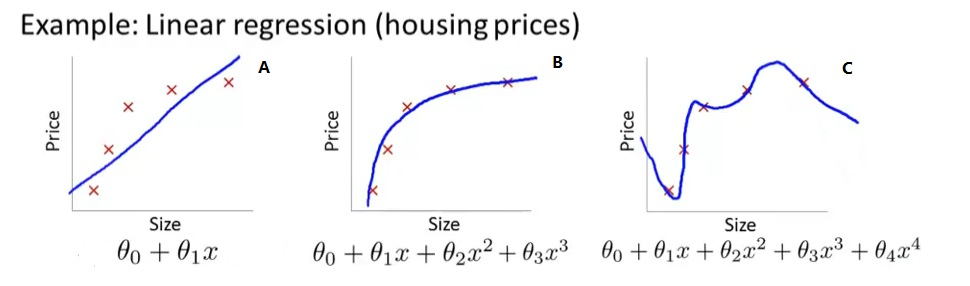
\includegraphics[width=10cm]{Figure1.jpg}\\
  \caption{}\label{over-fitting_linear_regression_example}
\end{figure}

\begin{figure}[ht]
  \centering
  % Requires \usepackage{graphicx}
  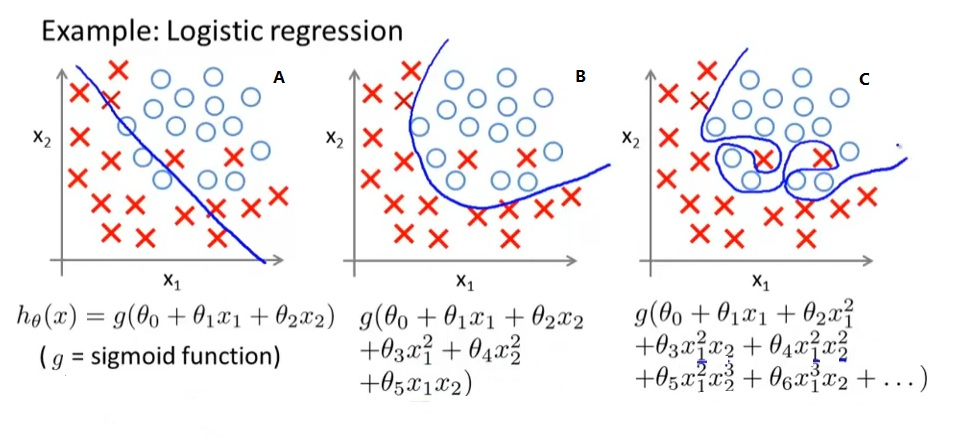
\includegraphics[width=10cm]{Figure2.jpg}\\
  \caption{}\label{over-fitting_logistic_regression_example}
\end{figure}

\section{Regularized Cost Function}
The intuition of regularization is to penalize large parameters of $\Theta$ and keep the hypothesis simple. In Fig. \ref{over-fitting_linear_regression_example}C, if we can penalize $\Theta_{4}$ and shrink it to zero, the hypothesis will much closer to the "right" one. Regularization adds a term of $\frac{\lambda}{2m} \sum_{j=1}^{n}\Theta_{j}^{2}$ to the regression cost function. So, the new cost function is as (\ref{regular_cost_function}).
\begin{equation}\label{regular_cost_function}
J^{'}(\Theta) = J(\Theta) + \frac{\lambda}{2m} \sum_{j=1}^{n}\Theta_{j}^{2}
\end{equation}
The larger value of $\Theta_{j}$, the larger cost of the corresponding hypothesis, hence the gradient descent algorithm will penalize large $\Theta_{j}$. Note j starts from 1 instead of 0, it is because $\Theta_{0}$ is the const value of the hypothesis function and does not influence the complexity.

\section{Regularized Gradient Descent}
Calculating the partial derivatives of (\ref{regular_cost_function}) for each of $\theta_{j}$, we can infer the regularized gradient descent for regression problem. The only difference of regularized gradient descent for linear regression and logistic regression is the hypothesis function.
\smallskip
\hrule
\smallskip
Algorithm1: Regularized Gradient Descent for Regression Problem
\smallskip
\hrule
\smallskip
Repeat\{\\
$\Theta_0=\Theta_0 - \alpha \frac{1}{m} \sum_{i=1}^{m}(h_\Theta(x^{(i)})-y^{(i)}) \cdot x^{(i)}_{0}$\\
$\Theta_j=\Theta_j(1 - \frac{\lambda}{\alpha m}) - \alpha \frac{1}{m} \sum_{i=1}^{m}(h_\Theta(x^{(i)})-y^{(i)}) \cdot x^{(i)}_{j}$ (j=1 \ldots n)\\
\}\\
\hrule
\section{Regularized Normal Equation}
Normal equation is an alternative for solving linear regression problem. All $\Theta s$ can be calculated by a system of linear equations. When using the new regularized cost function shown in (\ref{regular_cost_function}), we have the regularized normal equation shown in (\ref{regularized_normal_euqation}).
\begin{equation}\label{regularized_normal_euqation}
\Theta = (X^{T}X + \lambda(I_{n+1} - e_{0}))^{-1}X^{T}Y
\end{equation}
In (\ref{regularized_normal_euqation}), $I_{n}$ is n $\times$ n dimensional elementary matrix and $e_{0}$ equals $[1 \quad 0 \ldots 0]_{1 \times (n+1)}^{T}$.

\section{Summary}
Over-fitting is a common problem when using machine learning algorithms. Regularization penalizes large $\Theta s$ and keep the hypothesis simple to overcome this problem. In practice, regularization produces good outcome.
\end{document}
